\chapter{数据来源}
本课设的特色指出在于使用学界公认的数据MNIST和自制多种的数据, 通过的不同的数据,
相同或者相似的网络来处理这些数据, 然后比对结果, 所以数据的特点的理解是下一步实
现的基础。

\section{MNIST}

MNIST数据集是公认的较为可信的入门级的数据集, 当深度学习没有流行的时候,传统的
机器学习方法已经可以在MNIST上实现较为良好的结果。MNIST的所有图片$28 * 28$的大小
,数字分别标签为0到9,图\ref{mnist-data-1} 图\ref{mnist-data-2}分别是MNIST数据中
间的两种形态的2, 图\ref{mnist-data-3}是MNIST数据集中9。MNIST的测试数据和训练数据
一共含有60000张。 猜测可能是由于的MNIST中间的数据更加多以及其中的数据的识别标准
更加宽容,最终在MNIST上的数据的结果总是最佳的。
\begin{figure}[!hbt]
    \centering
    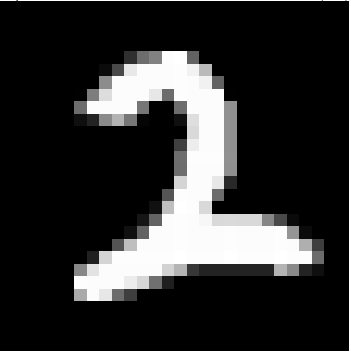
\includegraphics[width=0.3\linewidth]{pic/mnist-data-a.png}
    \caption{手写字2}
    \label{mnist-data-1}
\end{figure}

\begin{figure}[!hbt]
    \centering
    
\includegraphics[width=0.3\linewidth]{pic/mnist-data-b.png}
    \caption{手写字2}
    \label{mnist-data-2}
\end{figure}

\begin{figure}[!hbt]
    \centering
    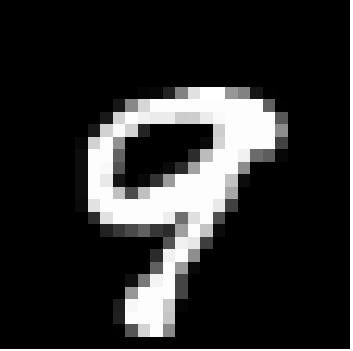
\includegraphics[width=0.3\linewidth]{pic/mnist-data-c.png}
    \caption{手写字9}
    \label{mnist-data-3}
\end{figure}

\section{线条}
此数据是使用python的工具绘制出来的数据, 在本数据集合中间,图片的大小是60 * 60
的大小, 图片中间线条的数目从0到9各有1000张, 一共含有10000张图片。
图\ref{line-data-1} 和 图\ref{line-data-2} 展示的其中的两个样张。
\begin{figure}[!hbt]
    \centering
    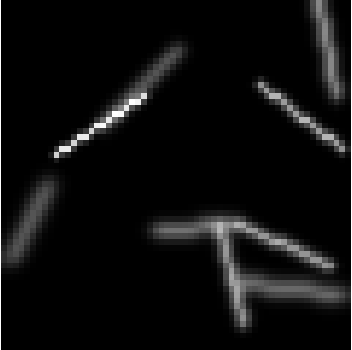
\includegraphics[width=0.3\linewidth]{pic/line-data-a.png}
    \caption{含有9个线条}
    \label{line-data-1}
\end{figure}

\begin{figure}[!hbt]
    \centering
    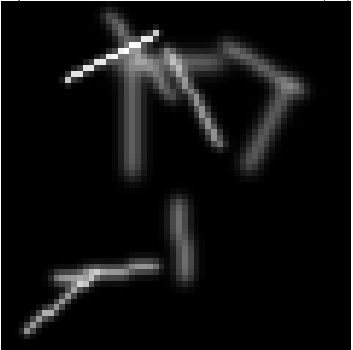
\includegraphics[width=0.3\linewidth]{pic/line-data-b.png}
    \caption{含有10个线条}
    \label{line-data-2}
\end{figure}

\section{拼图}
在此处的拼图的定义是图像中间含有两个由一个矩形拆分成得到的两个部分。
\ref{tile-data-a} 和\ref{tile-data-b}显示的其中的两个样张。每一张图片的大小是28
* 28, 一共含有10000张图片。
\begin{figure}[!hbt]
    \centering
    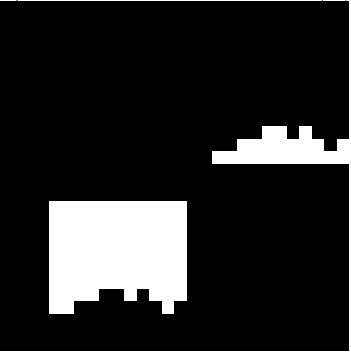
\includegraphics[width=0.3\linewidth]{pic/tile-data-a.png}
    \caption{拼图1}
    \label{tile-data-a}
\end{figure}

\begin{figure}[!hbt]
    \centering
    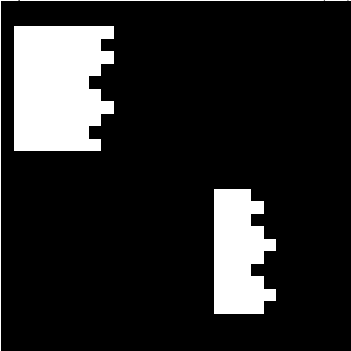
\includegraphics[width=0.3\linewidth]{pic/tile-data-b.png}
    \caption{拼图2}
    \label{tile-data-b}
\end{figure}

\section{正多边形}
正多边形是从三角形, 正方形等一直到正十二边形, 相同的图形在在其中含有旋转, 大
小和中心位置的不同等区别。\ref{polygon-data-a}和\ref{polygon-data-b}是两个不同的
三角形, 其旋转方向不相同。
\ref{polygon-data-c}是正十边形。

\begin{figure}[!hbt]
    \centering
    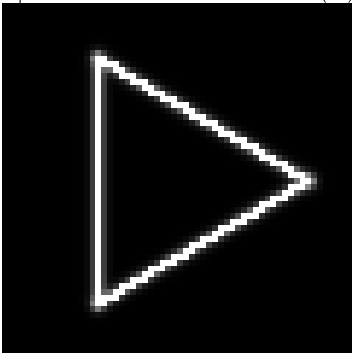
\includegraphics[width=0.3\linewidth]{pic/polygon-data-a.png}
    \caption{拼图1}
    \label{polygon-data-a}
\end{figure}

\begin{figure}[!hbt]
    \centering
    
\includegraphics[width=0.3\linewidth]{pic/polygon-data-b.png}
    \caption{三角形}
    \label{polygon-data-b}
\end{figure}

\begin{figure}[!hbt]
    \centering
    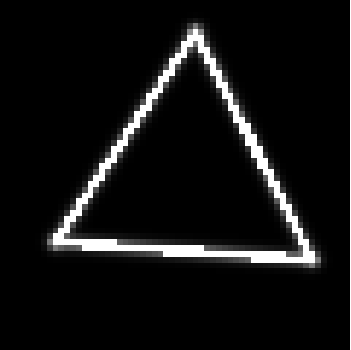
\includegraphics[width=0.3\linewidth]{pic/polygon-data-c.png}
    \caption{正十边形}
    \label{polygon-data-b}
\end{figure}

\section{点}

点图形指的是\ref{star-data-a}以及\ref{star-data-b}类似,每一张图片包含的十字状的
物体若干个,数目从0到9不等,一共含有10000张图片, 图片的大小是28 * 28.

\begin{figure}[!hbt]
    \centering
    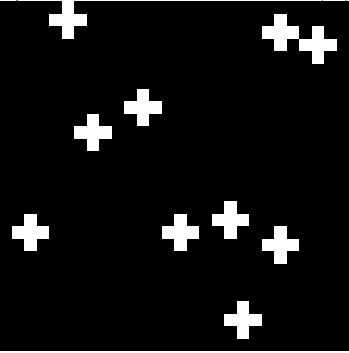
\includegraphics[width=0.3\linewidth]{pic/star-data-a.png}
    \caption{包含四个点}
    \label{star-data-a}
\end{figure}

\begin{figure}[!hbt]
    \centering
    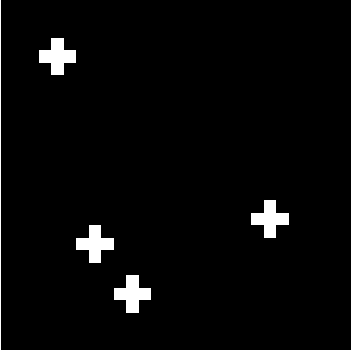
\includegraphics[width=0.3\linewidth]{pic/star-data-b.png}
    \caption{包含十个点}
    \label{star-data-b}
\end{figure}

\section{数据来源总结}
\ref{data_table_1}展示全部数据的总结, 需要说明一下为何处理正多边形的数目是800而
不是10000, 主要原因是绘制的正多边形的算法的实现导致想要得到10000张图片需要非常长
的时间,除此之外,正多边形的图片之间的变化更加小, 所以绘制比较少。
\begin{table}[htb]
\centering
\label{data_table_1}
\begin{tabular}{c|c|c|c}
\hline\hline

\textbf{名称} & \textbf{图片大小} & \textbf{图片数目} & \textbf{数据是否自制} \\
\hline\hline

MNIST    & 28 * 28 & 60000  & 否\\
\hline

线条     & 60 * 60 & 10000  & 是 \\
\hline

拼图     & 28 * 28 & 100000 & 是 \\
\hline

正多边形 & 60 * 60 & 800    & 是\\
\hline

点       & 28 * 28 & 10000  & 是 \\
\hline

\hline\hline
\end{tabular}
\caption{各节点硬件配置要求}
\end{table}

